\section{Programmable Storage}
\label{sec:progly}

When application requirements are not met by an underlying storage system the
most common approach is to design workarounds that roughly fall into one
of three categories:

{\bf Extra services.} ``Bolt-on'' services are intended to improve performance
or enable a feature, but come at the expense of additional hardware, software
sub-systems, and dependencies that must be managed, as well as trusted.
For instance, many extensions to Hadoop have been created to address its
limitations~\cite{bu:vldb2010-haloop, ekanayake:hpdc2010-twister,
ekanayake:escience2008-eglmapreduce, mihailescu:hotstorage2012-mixapart}.

{\bf Application changes.} The second approach to adapting to a storage system
deficiency is to change the application itself by adding more data management
intelligence into the application or as domain-specific middleware. When
application changes depend on non-standard semantics exposed by the storage
system (e.g. relaxed POSIX file I/O or MPI-IO hints) the coupling that results
can be fragile.
For example, \cite{buck:hpc2011-scihadoop, gkantsidis:nsdi2013-rhea} both do
an excellent jobs of partitioning data in Hadoop applications, but may not
stand the test of time for future workloads, since the partitioning is
specific to scientific data.

{\bf Storage modifications.} When these two approaches fail to meet an
application's needs, developers may turn their attention to any number of
heavy-weight solutions ranging from changing the storage system itself, up to
and including designing entirely new systems. This approach can require
significant cost, domain knowledge, and extreme care when building or
modifying critical software that can take years of code-hardening to trust.
For example, HDFS fails to meet many needs 
of metadata-intensive workloads~\cite{shvachko:login2012-hdfs-scalability}.
This has lead to modifications to its architecture or
API~\cite{balmin:sigmod2012-clydesdale} to improve performance.

Rather than relying on storage systems to evolve \emph{or} applications to
change, a hybrid approach that embraces interface instability allows maximum
flexibility, so long as it does not impose an unmanageable burden on
developers.

\subsection{The Malacology Approach}

Malacology is a recently proposed approach to co-design between applications
and storage systems that advocates a design strategy called programmable
storage in which existing storage system services are safely exposed such that
they can be composed to form application specific
services~\cite{msevilla:eurosys17}.
Figure~\ref{fig:malacology} shows the architecture of Malacology as
implemented in Ceph, which exposes a variety of low-level internal services
such custom object interfaces, cluster metadata management, and
load-balancing. While Ceph natively exposes file, block, and object
abstractions, Malacology demonstrated the construction of two real-world
services using only a combination of existing interfaces present in Ceph.

\begin{figure}[t]
\centering
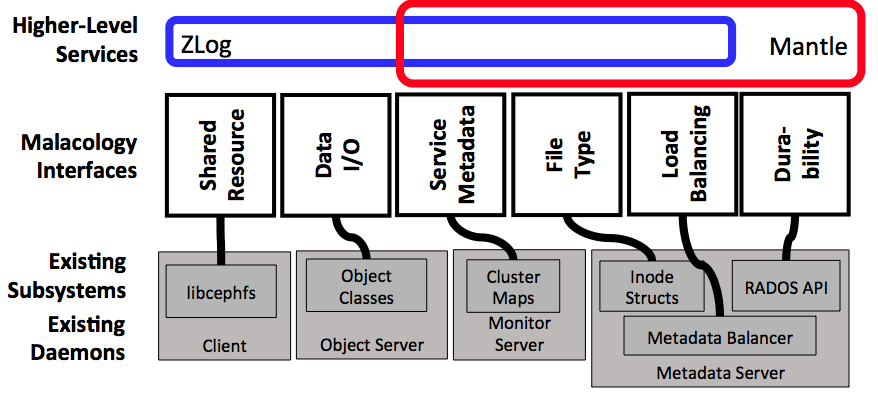
\includegraphics[width=1.0\linewidth]{implementation-overview.png}
\caption{Malacology implementation in Ceph. Existing sub-systems are composed
    to form new services and application-specific optimizations.}
\label{fig:malacology}
\end{figure}

One of these synthesized interface is a high-performanced distributed shared
log that implements the CORFU protocol~\cite{balakrishnan:nsdi12}.
This protocol achieves high-throughput
using a network-attached
counter for high-frequency log position assignment, and depends on a custom
storage device interface that exposes a write-once infinite address space that
is critical to maintaining correctness across faults and reconfiguration.
Malacology reproduces the CORFU
network-attached counter service using a capability-based mechanism found in
the Ceph distributed file system for managing cached metadata. The service
models the counter state as temporary exclusive access to file metadata.
The storage device interface in
CORFU is constructed using a software abstraction that maintains consistency
across independent low-level Ceph I/O interfaces such as indexes and
bytestreams.

The demonstration of interface synthesis in Malacology suggests a new form of
application development that significantly reduces the programming surface
area. While this ability to construct software-defined interfaces is powerful,
next we will show how access to low-level interfaces can be a double-edged
sword, providing its power at the cost of maintenance complexity.
